\chapter{Introducción a Teoría de Grafos}

\section{Grafos}

\subsection{Definición}

Un \textit{grafo} es un par ordenado $G = (V, E)$: el conjunto $V$, de \textit{vértices} o \textit{nodos} , y el de aristas/arcos $E$, que relacionan a esos nodos.

En el caso de los grafos \textit{no dirigidos} (o simplemente grafos), $E \subseteq \{\{v_1, v_2\}\ |\ v_1,v_2 \in V, v_1 \neq v_2 \}$ es un conjunto de pares no ordenados de los elementos de $V$, conocidos como \textit{aristas}. Por otro lado, para los \textit{grafos dirigidos} (también llamados \textit{digrafos}), $E \subseteq V \times V$ tiene pares ordenados de nodos, y sus elementos se denominan arcos. Se suele realizar un abuso de notación menor, utilizando $(v, w)$ para referirse tanto a aristas como arcos.

\begin{figure}[H]
    \centering
    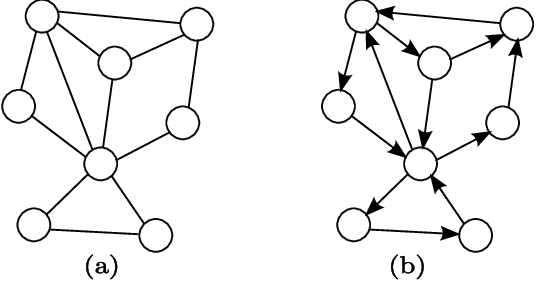
\includegraphics[width=0.5\textwidth]{ejemplo_grafo.png}
    \small
    \caption*{Representaciones gráficas de un grafo (a) y un digrafo (b). Los círculos son los vértices, y las líneas/flechas son las aristas/arcos.}
\end{figure}

En general, se denota $n_G = |V|$ y $m_G = |E|$ para referirse a las cantidades de vértices y aristas. Cuando el grafo referido es inambigüo, se omite el subíndice\footnote{Lo mismo vale para el resto de las definiciones en esta sección.}.

\subsection{Vecinos}

Dados $v,w \in V$, se denominan \textit{adyacentes} cuando $e = (v,w) \in E$, y que $e$ es \textit{incidente} a $v$ y $w$. Similarmente, la \textit{vecindad} de $v$, denotada por $N_G(v)$ es el conjunto de vértices adyacentes a $v$, es decir:
$$N_G(v) = \{w \in V \mid (v, w) \in E\}$$

Por otro lado, la cantidad de aristas incidentes a un vértice $v$ se llama \textit{grado}, definida como:
$$d_G(v) = |N_G(v)|$$

\begin{theorem*}
    Dado un grafo de $G = (V, E)$, la suma de los grados de sus vértices es el doble de la cantidad de aristas. Es decir,
    $$\sum_{v \in V} d(v) = 2m$$
\end{theorem*}
\begin{proof}
    Se puede demostrar por inducción en $m$, la cantidad de aristas.

    \textbf{Caso base:} Se puede tomar como caso base $m = 0$. En un grafo sin aristas, todos los vértices tienen grado $0$, y por ende:
    $$\sum_{v \in V} d(v) = 0 = 2m$$

    \textbf{Paso inductivo:} Asumiendo que la propiedad se cumple para $m = k$, tomemos un grafo cualquiera $G = (V, E)$ con $|E| = k + 1$ aristas. Se puede elegir una arista cualquiera $e = (v, w) \in E$, y construir el grafo $G' = (V, E - {e})$ que resulta de quitar una de sus aristas. Como $m_{G'} = k$, se cumple la hipótesis inductiva:
    $$\sum_{u \in V} d_{G'}(u) = 2m_{G'} = 2k$$

    Luego, para el grafo original $G$, la adición de la arista $e$ solo incrementea el grado de los vértices $v$ y $w$. Concretamente:
    $$
        d_G(u) =
        \begin{cases}
            d_{G'}(u) + 1 & \si u = v \lor u = w \\
            d_{G'}(u)     & \ecc
        \end{cases}
    $$
    Por lo tanto, se tiene:
    \begin{align*}
        \sum_{u \in V} d_G(u) & = \sum_{v \in V - \{v, w\}} d_{G'}(u) + (d_{G'}(v) + 1) + (d_{G'}(w) + 1) \\
                              & = \sum_{u \in V} d_{G'}(u) + 2 \stackrel{HI}{=} 2k + 2 = 2(k + 1) = 2m_G
    \end{align*}

    Lo cual, por inducción, implica que la propiedad vale para todo $m \in \N$.

\end{proof}

\subsubsection{Complemento}

Dado un grafo $G = (V, E)$, su \textit{grafo complemento}, denotado como $\bar{G} = (V, \bar{E})$, tiene el mismo conjunto de vértices, pero cada par de vértices es adyacente en $\bar{G}$ si y solo si no lo es en $G$. Es decir,
$$\bar{E} = (V \times V) - E$$

\subsubsection{Grafos Completos}

El grafo $K_n$ es el \textit{grafo completo} de $n$ vértices, los cuales son todos adyacentes entre sí. Este grafo tiene $m_{K_n} = \frac{n(n-1)}{2}$.

\begin{figure}[H]
    \centering
    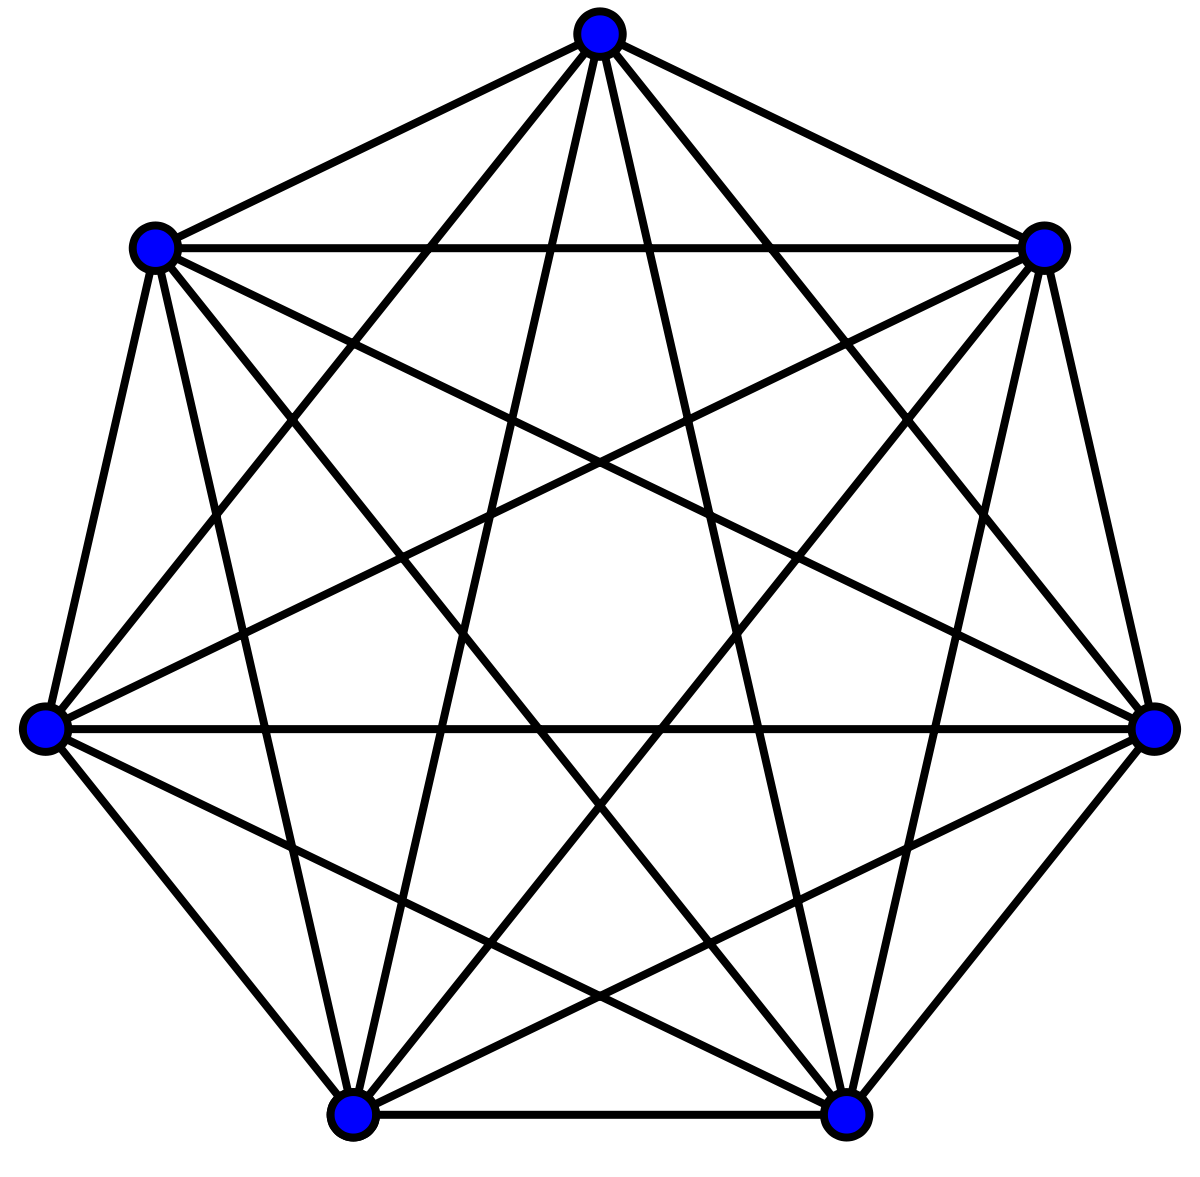
\includegraphics[width=0.3\textwidth]{K7.png}
    \caption*{Representación gráfica del grafo completo $K_7$.}
\end{figure}

\subsection{Generalizaciones}

Algunas generalizaciones\footnote{No se estudian mucho en la materia.} de los grafos son:
\begin{itemize}
    \item \textbf{Multigrafos}: En un multigrafo, $E$ pasa a ser un multiconjunto, es decir, pueden haber varias aristas entre un mismo par de vértices.
    \item \textbf{Pseudografo}: Los pseudografos pueden tiene varias aristas entre un mismo par de vértices, y también puede haber aristas que unan a un mismo par de vértices (llamadas \textit{loops}).
\end{itemize}

\subsection{Recorridos}

\begin{itemize}
    \item Un \textit{recorrido} en un grafo es una secuencia de vértices $P = v_0 v_1 \cdots v_k$ tal que todos los pares consecutivos son adyacentes, es decir, $(v_i, v_{i+1}) \in E\ \forall i = 0, ..., k - 1$. Para multi- y pseudo-grafos, se debe especificar entre qué aristas se pasa.
    \item Un \textit{camino}\footnote{Hay ambigüedad en el término: a veces se llama camino a los recorridos, en cuyo caso a los recorridos sin vértices repetidos se les dice \textit{camino simple}.} es un recorrido que no pasa por el mismo vértice $2$ veces.
    \item Una \textit{sección} de un recorrido $P$ es una subsecuencia $S = v_i v_{i+1} \cdots v_j$ de vértices consecutivos de $P$, y se denota $P_{v_i v_j}$.
    \item Un \textit{circuito} es un recorrido que empieza y termina en el mismo vértice.
    \item Un \textit{ciclo} o \textit{circuito simple} es un circuito de $3$ o más vértices que no pasa $2$ veces por el mismo vértice (salvo por el principio y fin).
\end{itemize}

\begin{figure}[H]
    \centering
    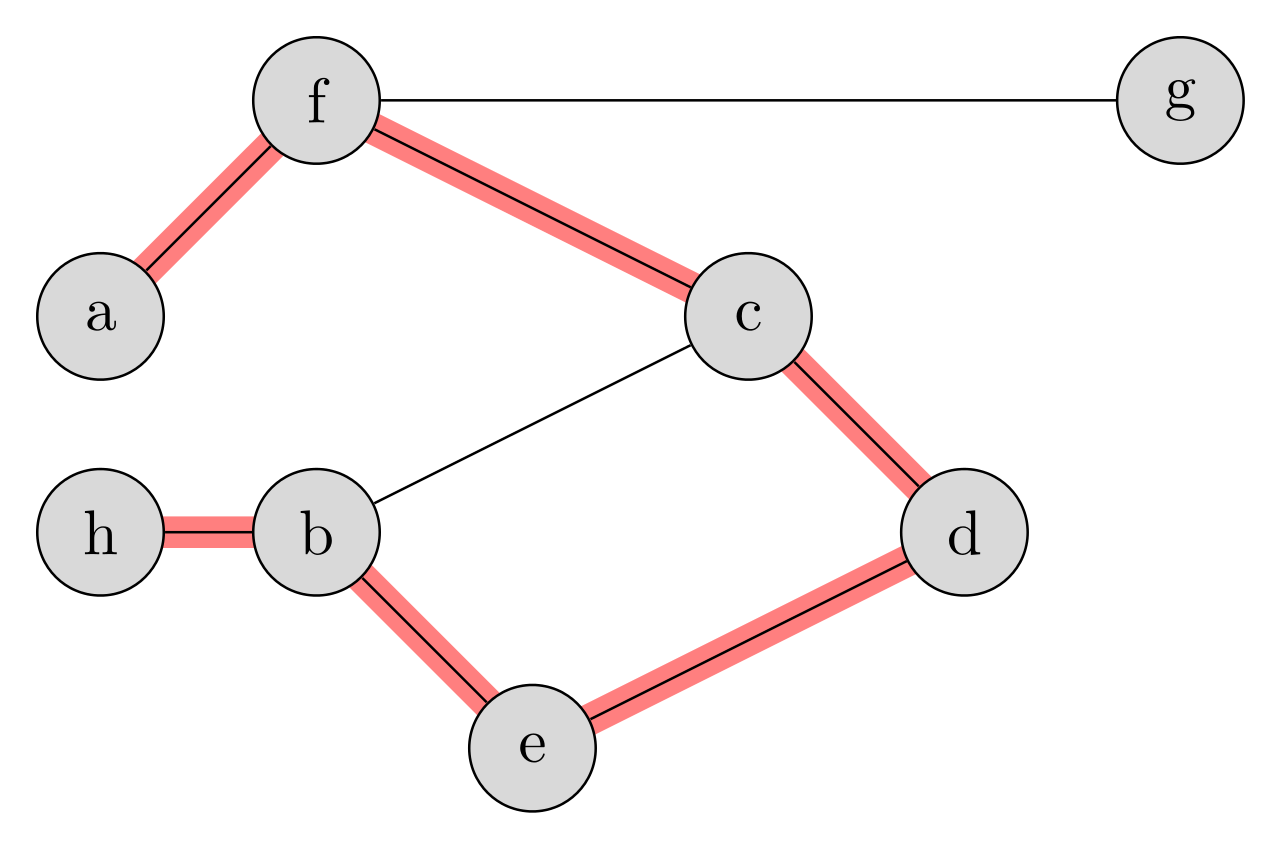
\includegraphics[width=0.3\textwidth]{ejemplo_camino.png}
    \caption*{Un ejemplo de un camino entre los vértices $a$ y $h$.}
\end{figure}

\subsection{Distancia}

Dado un recorrido $P$, su \textit{longitud}, $l(P)$, es la cantidad de aristas que tiene. Luego, la \textit{distancia} entre $v$ y $w$ se define como la longitud del camino más corto entre $v$ y $w$, y se llama $d(v, w)$. Si no hay recorrido entre $v$ y $w$, se define que $d(v, w) = \infty$, mientras que $d(v, v) = 0$ para cualquier $v$.

\begin{theorem*}
    Si un recorrido $P$ entre $v$ y $w$ cumple $l(P) = d(v, w)$, entonces es un camino.
\end{theorem*}
\begin{proof}
    Se puede demostrar por el absurdo: si $P$ no fuera un camino, tendría algún vértice $u$ por el que se pasa $2$ veces: $P = v \cdots u \cdots u \cdots w$. Si se forma un nuevo recorrido $P' = P_{vu} + P_{uw}$ (excluyendo el recorrido de $u$ a sí mismo), este tendría una longitud estrictamente menor que $P$, y por ende $l(P') < d(v, w)$ (\textbf{Absurdo}).

\end{proof}

\begin{theorem*}
    Para cualquier grafo $G = (V, E)$, la función de distancia $d: V \times V \longrightarrow \N$ es una métrica, es decir, cumple las siguientes propiedades para todo $u, v, w \in V$:
    \begin{itemize}
        \item $d(u, v) = 0 \iff u = v$
        \item $d(u, v) = d(v, u)$
        \item $d(u, w) \leq d(u, v) + d(v, w)$ (desigualdad triangular)
    \end{itemize}
\end{theorem*}
\begin{proof}
    Se demuestra por separado:
    \begin{itemize}
        \item La ida vale por definición, y la vuelta vale porque cualquier camino entre un par de vértices tiene al menos $1$ arista (y por ende $d(u, v) \geq 1$).
        \item En un grafo las aristas no tienen sentido, así que cualquier camino puede ser invertido para formar un camino válido. Por ende, la longitud del camino más corto entre $u$ y $v$ debe ser la misma que entre $v$ y $u$.
        \item Si $P_{uv}$ y $P_{vw}$ son caminos tales que $l(P_{uv}) = d(u,v)$ y $l(P_{vw}) = d(v,w)$, se pueden concatenar para formar un recorrido $P_{uv} + P_{vw}$ entre $u$ y $w$. Como la distancia es la longitud mínima entre todos los recorridos, se tiene $d(u, w) \leq l(P_{uv} + P_{vw}) = d(u, v) + d(v, w)$.
    \end{itemize}

\end{proof}

\subsection{Subgrafos}
\label{subgrafos}

Dado un grafo $G = (V_G, E_G)$,

\begin{itemize}
    \item Un \textit{subgrafo} de $G$ es un grafo $H = (V_H, E_H)$ tal que $V_H \subseteq V_G$ y $E_H \subseteq E_G \cap (V_H \times V_H)$. Los notamos como $H \subseteq G$.
    \item $H$ es un \textit{subgrafo propio} cuando $H \subseteq G$ y $H \neq G$.
    \item $H$ es un \textit{subgrafo generador} cuando $H \subseteq G$ y $V_H = V_G$.
    \item $H$ es un \textit{subgrafo inducido} cuando $(v, w) \in E_H \iff v,w \in V_H \land (v, w) \in E_H$. Estos subgrafos pueden definirse únicamente por su conjunto de vértices, y se denota como $G_{[V_H]}$.
\end{itemize}

\subsection{Conectividad}

Un grafo se denomina \textit{conexo} cuando existe un camino entre todo par de vértices. Una \textit{componente conexa} de un grafo es un subgrafo inducido conexo maximal (no se pueden agregar más vértices y mantenerlo conexo) de $G$.

Por otro lado, una arista de $G$ es \textit{puente} si $G - e$ tiene más componentes conexas que $G$.

\begin{figure}[H]
    \centering
    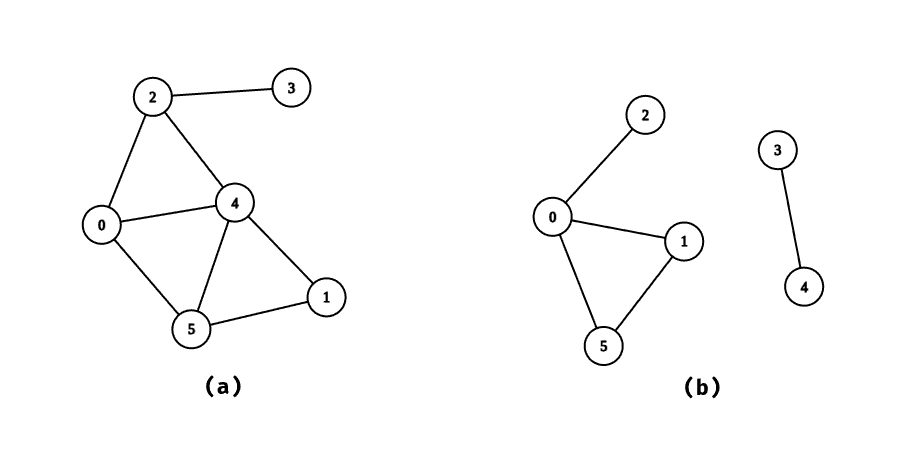
\includegraphics[width=0.5\textwidth]{ejemplo_conexo.png}
    \caption*{Un grafo conexo (a) y uno disconexo (b).}
\end{figure}

\subsection{Representación de Grafos}
\label{representacion-grafos}

Existen distintas alternativas para representar grafos en un algoritmo, que proveen ventajas y desventajas a la hora de realizar diversas operaciones.

\subsubsection{Lista de aristas}

El grafo se almacena como una lista de pares de vértices, que representan sus aristas. Esta es la forma más simple de representarlo, y es el formato que se asume que tiene la entrada de cualquier algoritmo de grafos. Debido a su falta de estructura, realizar la mayoría de las operaciones resulta costoso, con la excepción de agregar nodos o aristas.

Esta estructura tiene ciertas variaciones. Por ejemplo, se pueden ordenar los vértices dentro de cada lista, lo cual permite usar búsqueda binaria para comprobar la pertenencia de un vértice a ellas, pero aumenta la complejidad de construir la estructura y la de agregar vértices (porque hay que mantener el orden).

\subsubsection{Listas de adyacencia}

Se mantienen $n$ listas, donde cada lista $L_i$ contiene todos los vértices de $N(v_i)$. Esto permite realizar algunas operaciones más rápidamente, y la estructura se puede construir a partir de la lista de aristas en tiempo lineal.

\subsubsection{Matriz de adyacencia}

En este caso, se tiene una matriz $M \in \{0, 1\}^{n \times n}$, donde cada posición está determinada por:
$$
    M_ij =
    \begin{cases}
        1 & \si (i, j) \in E \\
        0 & \ecc
    \end{cases}
$$

La matriz es simétrica para grafos, pero no necesariamente para digrafos.

La estructura permite comprobar si dos vértices son adyacentes en tiempo constante. Sin embargo, construirla a partir de una lista de adyacencia es una operación de complejidad cuadrática, y la estructura es muy rígida (para agregar un vértice se debe armar una nueva matriz). Además, la complejidad espacial es también \BigO{|V|^2}, lo cual es problemático para guardar grafos ralos\footnote{Un grafo \textit{ralo} es uno con ``pocas'' aristas.}.

\subsubsection{Matriz de incidencia}

Esta estructura es una matriz $I \in \{0, 1\}^{m \times n}$ donde las filas representan los vértices y las columnas las aristas. Una posición $i, j$ tiene uno cuando la arista de la columna $j$ es incidente al vértice de la fila $i$.

\subsubsection{Complejidades}

% TODO: Tabla de complejidades

\subsection{Isomorfismo}

Dos grafos $G = (V, E)$ y $G' = (V', E')$ son \textit{isomorfos} cuando existe una función biyectiva $f: V \longrightarrow V'$ tal que:
$$\forall v, w \in V,\ (v, w) \in E \iff (f(v), f(w)) \in E'$$

A la función $f$ se la llama isomorfismo, y se denota $G \approxeq G'$ o (por abuso de notación) $G = G'$.

\begin{theorem*}
    Si dos grafos $G \approxeq G'$ son isomorfos.
    \begin{itemize}
        \item Tienen el mismo número de vértices.
        \item Tiene el mismo número de aristas.
        \item $\forall 0 \leq k \leq n - 1,$ tienen el mismo número de vértices de grado $k$.
        \item Tienen el mismo número de componentes conexas.
        \item $\forall 0 \leq k \leq n - 1,$ tienen el mismo número de caminos simples de longitud $k$.
    \end{itemize}
\end{theorem*}
\begin{proof}
    % TODO

\end{proof}

\subsection{Definiciones en digrafos}

\subsubsection{Vecinos}

\begin{itemize}
    \item Para un arco $e = (v, w) = v \rightarrow w$, se llama \textit{cola} de $e$ a $v$ y \textit{cabeza} de $e$ a $w$.
    \item El \textit{grado de entrada} $d_-(v)$ es la cantidad de arcos que tienen a $v$ como cabeza.
    \item El \textit{grado de salida} $d_+(v)$ es la cantidad de arcos que tienen a $v$ como cola.
    \item El \textit{grafo subyacente} de $G$ es el grafo que resulta de ignorar las direcciones de sus arcos.
\end{itemize}

\subsubsection{Recorridos}
\label{recorridos-digrafos}

\begin{itemize}
    \item Un \textit{recorrido/camino orientado} en un digrafo es una sucesión de vértices que están conectados apropiadamente por arcos (sin repetidos en el caso del camino).
    \item Un \textit{circuito/ciclo orientado} es un recorrido/camino orientado que empieza y termina en el mismo vértice.
    \item Un digrafo es \textit{fuertemente conexo} si para todo par de vértices $v, u$ existen caminos orientados de $u$ a $v$ y de $v$ a $u$.
\end{itemize}

\section{Grafos Bipartitos}

Un grafo $G = (V, E)$ es \textit{bipartito} cuando existe una \textit{bipartición} de sus vértices $(V_1, V_2)$ tal que todas las aristas de $G$ tienen un extremo en $V_1$ y el otro en $V_2$. Por otro lado, $G$ es \textit{bipartito completo} cuando todo vértice de $V_1$ es adyacente a todo vértice de $V_2$, y se denota $G = K_{|V_1|,|V_2|}$.

\begin{figure}[H]
    \centering
    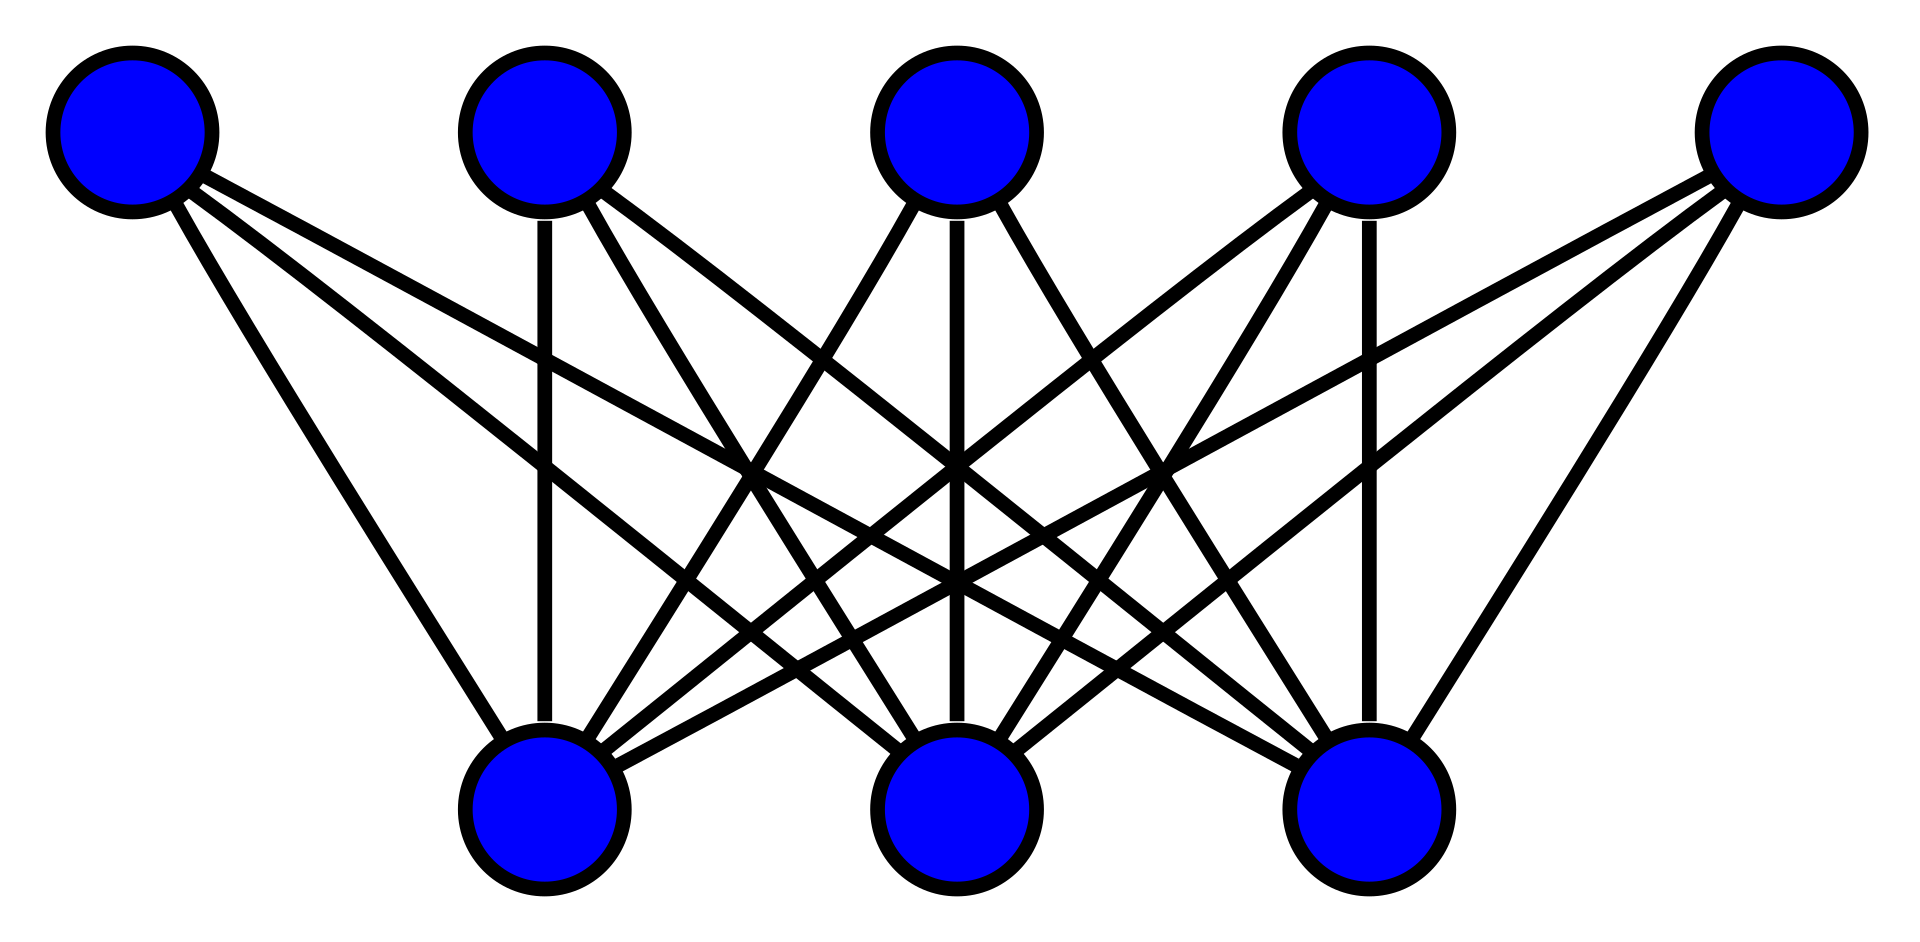
\includegraphics[width=0.3\textwidth]{grafo_K_3,5.png}
    \caption*{El grafo bipartito completo $K_{3,5}$.}
\end{figure}

\begin{theorem*}
    Un grafo $G$ es bipartito $\iff$ no tiene ciclos de longitud impar.
\end{theorem*}
\begin{proof}
    Como un grafo es bipartito si y solo si cada una de sus componentes conexas es bipartita, y un grafo no tiene ciclos impares si y solo si ninguna de sus componentes conexas tiene ciclos impares, alcanza con demostrar el teorema para grafos conexos.

    $\implies$) Sea $(V_1, V_2)$ la bipartición de $G$.

    Si $G$ tiene algún ciclo $C = v_1v_2 \cdots v_kv_1$, se puede asumir sin pérdida de generalidad que $v_1 \in V_1$. Luego, como $v_1v_2 \in E$ (y $G$ es bipartito), $v_2 \in V_2$. En general, $v_{2i+1} \in V_1$ y $v_{2i} \in V_2$. Como $v_1 \in V_1$ y $v_kv_1 \in E$, se debe cumplir $v_k \in V_2$. Por ende $k = 2i$ así que $l(C)$ es par.

    $\impliedby$) Sea $u$ cualquier vértice de $V$. Se definen los siguientes conjuntos:
    \begin{align*}
        V_1 & = \{v \in V \mid 2 \mid d(u, v)\} \cup \{u\} \\
        V_2 & = \{v \in V \mid 2 \nmid d(u, v)\}
    \end{align*}

    $(V_1,V_2)$ definen una partición de $V$. Se puede demostrar que es una bipartición de $G$ por el absurdo.

    Supongamos que no es una bipartición, entonces existen $v, w \in V_1$ (s.p.g.) tales que $vw \in E$. Si $v = u$, entonces $d(v,u) = 1$, que es absurdo porque $d(v, w)$ es par. Lo mismo vale para $w$, así que $v \neq u$ y $v \neq w$.

    Sea $P$ un camino mínimo entre $v$ y $u$ y $Q$ uno entre $v$ y $w$. Como $u, w \in V_1$ $P$ y $Q$ tienen longitud par. Luego, sea $z$ el vértice común a $P$ y $Q$ tal que $P_{zv}$ y $Q_{zw}$ son disjuntos (ignorando $z$).

    Se debe cumplir $d(u, z) = l(P_{uz}) = l(Q_{uz})$, porque del contrario $P$ y $Q$ no serían caminos mínimos. Esto implica que $l(P_{zv})$ y $l(Q_{zw})$ tienen la misma paridad, porque $l(P)$ y $l(Q)$ son ambos pares y la diferencia entre las longitudes totales y las de los subcaminos es la misma. Por ende, el ciclo $P_{zv}(v, w)Q_{wz}$ tiene longitud impar (\textbf{Absurdo}).

\end{proof}

\section{Árboles}

\subsection{Definición}

Un \textit{árbol} es un grafo conexo acíclico.

\begin{figure}[H]
    \centering
    \includegraphics*[width=0.5\textwidth]{ejemplos_arboles.png}
    \caption*{Ejemplos de grafos que son árboles.}
\end{figure}

Existen caracterizaciones alternativas:

\begin{theorem*}
    Dado un grafo $G = (V, E)$, son equivalentes:
    \begin{enumerate}
        \item G es un árbol (un grafo conexo acíclico).
        \item G es un grafo acíclico y $\forall e \notin X,$ $G + e = (V, E \cup \{e\})$ tiene exáctamente un ciclo, y ese ciclo pasa por $e$.
        \item Existe exactamente un camino simple entre todo par de vértices de $G$.
        \item $G$ es conexo, pero si se quita cualquier arista de $G$, queda un grafo disconexo (toda arista es puente).
        \item $G$ es un grafo conexo con $|E| = |V| - 1$
        \item $G$ es un grafo acíclico con $|E| = |V| - 1$.
    \end{enumerate}
\end{theorem*}

% TODO (capaz): demostrar eso

\subsubsection{Hojas}

Una \textit{hoja} en un árbol es un vértice de grado $1$. Todo árbol \textit{no trivial} (con al menos $2$ vértices) tiene al menos $2$ hojas.

% TODO: Conseguir imagen
% \begin{figure}[H]
%     \centering
%     \includegraphics*[width=0.5\textwidth]{}
% \end{figure}

\subsubsection{Bosques}

Un \textit{bosque} es un grafo sin ciclos. Sus componentes conexas forman árboles, y se cumple $m = n - c$, donde $c$ es la cantidad de componentes conexas del bosque.

% TODO: Conseguir imagen

\subsection{Árboles enraizados}

Un \textit{árbol enraizado} es un árbol con un vértice especial $r$ designado \textit{raíz}. Luego, queda definido un árbol dirigido, donde los arcos van desde vértices más cercanos a la raíz hacia los más lejanos. En tal caso, está la siguiente terminología:
\begin{itemize}
    \item Los vértices \textit{internos} son aquellos que no son ni hojas ni raíz.
    \item El \textit{nivel} de un vértice $v$ es la distancia de la raíz a ese vértice ($d(r, v)$).
    \item Para cada arco $v \rightarrow w$, $v$ es el \textit{padre} de $w$, y $w$ es el \textit{hijo} de $v$.
    \item La \textit{altura} $h$ de un árbol enraizado es la distancia desde la raíz al vértice más lejano ($\max{\{d(r, v) \mid v \in V\}}$).
    \item Un árbol se dice \textit{$m$-ario} si todos sus nodos internos tiene grado a lo sumo $m + 1$ y la raíz tiene grado a lo sumo $m$.
    \item Un árbol es \textit{balanceado} cuando la diferencia entre el nivel de cada par de hojas es a lo sumo $1$.
\end{itemize}

\begin{theorem*}
    Dado un árbol enraizado $m$-ario con altura $h$ y $l$ hojas, $l \leq m^h$ ($\iff h \geq \lceil\log_m{l}\rceil$).
\end{theorem*}

% TODO: Demostración

\subsection{Representación de árboles}

Además de las representaciones de grafos \hyperref[representacion-grafos]{anteriormente mencionadas}, los árboles enraizados tienen una alternativa particular: debido a que todos los nodos tienen un único padre, un árbol puede ser definido por la correspondencia entre cada nodo y su antecesor. Esto se puede lograr usando solamente un arreglo ``\code{prev}'', en el que cada posición $i$ contiene al padre del nodo $v_i$. La única excepción es la raíz $r$ que, al no tener antecesor, se puede marcar utilizando un valor especial $\perp$, o como su propio padre ($d[r] = r$)\footnote{Esto se puede extender para guardar bosques: basta con tener varias raíces.}.

\subsection{Árbol generador}
\label{arbol-generador}

Un \textit{árbol generador} (AG) de un grafo $G$ es un \hyperref[subgrafos]{subgrafo generador} que además es un árbol. En la práctica, los árboles generadores son utilizados cuando se busca conectar (con la cantidad mínima posible de conexiones) a $n$ puntos (ciudades, centrales eléctricas, servidores).
\begin{theorem*}
    Dado un grafo conexo $G = (V, E)$.

    \begin{itemize}
        \item $G$ tiene (al menos) un árbol generador
        \item $G$ tiene un único árbol generador $\iff$ $G$ es un árbol.
        \item Sea $T = (V, E_T)$ un AG de $G$ y $e \in E - E_T$. Luego, para toda arista $f \neq e$ contenida en el único ciclo de $T + e$, $T + e - f = (V, E_T \cup \{e\} - \{f\})$ es un AG de $G$.
    \end{itemize}
\end{theorem*}

\section{Recorridos}
\label{recorridos}

Es común querer pasar por todos los vérices de un grafo una única vez. Existen distintos métodos de hacerlo de forma sistemática y ordenada, y en este caso nos vamos a enfocar en los $2$ más comunes: \textit{BFS} y \textit{DFS}. En ambos casos, se mantiene una \textit{frontera} con los vértices que se están por explorar, y cada vez que se pasa por uno de ellos sus vecinos son agregados a la misma. Además, se mantiene un conjunto de los vértices explorados (generalmente implementado con un \textit{bitset}) para evitar su repetición. El esquema general es el siguiente:

\begin{codebox}
    \Procname{$\proc{Recorrer}(G, s)$}
    \li Inicializar la frontera $F = \{s\}$.
    \li \While la frontera no esté vacía \Do
    \li Extraer un $v$ de la frontera.
    \li $\proc{Procesar}(v)$
    \li \For \Each $u \in N(v)$ \Do
    \li \If $u$ no fue visitado \Then
    \li Marcar a $u$ como visitado.
    \li Agregar $u$ a la frontera.
    \End
    \End
    \End
\end{codebox}

\subsection{BFS}

El \textit{Breadth-First Search} (BFS) es un algoritmo que, dado un grafo $G$ y un vértice inicial $s$, recorre todos los vértices nivel por nivel, es decir, los vértices más cercanos al inicial son visitados primero. Formalmente, si $\langle v_1, ..., v_n \rangle$ es la secuencia de vértices en el orden en que son recorridos, entonces se cumple:
$$d(s, v_i) \leq d(s, v_j)\ \forall\,1 \leq i \leq j \leq n$$

Para lograr esto, BFS utiliza como frontera una cola, donde los elementos son procesados en orden de llegada (FIFO). El algoritmo se puede implementar iterativamente de la siguiente manera:

\begin{codebox}
    \Procname{$\proc{BFS}(G = (V, E), s)$}
        \li $\id{visitados} \gets \emptyset$
        \li Inicializar árbol $T$ con raíz en $s$.
        \li Inicializar arreglo de distancias $d$.
        \li Inicializar cola $Q$.
        \li $d[s] \gets 0$
        \li $\proc{Encolar(Q, s)}$
        \li \While $\neg\proc{Vacío?}(Q)$ \Do
        \li $v \gets \proc{Desencolar}(Q)$
        \li $\proc{Procesar}(v)$
        \li \For \Each $u \in N(v)$ \Do
        \li \If $u \notin \id{visitados}$ \Then
        \li $\id{visitados} \gets \id{visitados} \cup \{u\}$
        \li $d[u] \gets d[v] + 1$
        \li Agregar $u$ a $T$ como hijo de $v$.
        \li $\proc{Encolar}(Q, u)$
        \End
        \End
        \End
        \li \Return $(T, d)$
\end{codebox}

El algoritmo devuelve $2$ valores: un árbol generador $T$, que se denomina \textit{árbol BFS} y contiene las aristas transitadas por el recorrido, junto con la función $d: V \longrightarrow \N_0$, que indica las distancias de $s$ a cada vértice del grafo.

Si el grafo se representa utilizando listas de adyacencia, el vecindario $N(v)$ se puede recorrer fácilmente. El algoritmo pasa una sola vez por cada vértice y, asumiendo que tanto $\id{visitados}$, $T$ y $d$ se representan a través arreglos, realiza una operación de tiempo constante en cada uno de sus vecinos. Por ende, la complejidad de este algoritmo es:
$$\BigO{|V| + \sum_{v \in V} d(v)} = \BigO{|V| + 2|E|} = \BigO{|V| + |E|}$$

\subsubsection{Árboles geodésicos}

Un árbol generador $T$ de un grafo $G$ se llama $v$-geodésico cuando $d_G(v, w) = d_T(v, w)\ \forall w \in V$.
\begin{theorem*}
    Si se corre el algoritmo BFS en un grafo $G$ empezando en un vértice $s$, el árbol generador resultante $T$ es $s$-geodésico, y las distancias que devuelve son las mínimas entre $s$ y cada vértice del árbol.
\end{theorem*}
\begin{proof}
    % TODO
\end{proof}

\subsection{DFS}

La estrategia que sigue el \textit{Depth-First Search} (DFS) es buscar ``en profundidad'' siempre que sea posible. Esto significa que al llegar a $v$, se recorren todos los vértices no visitados alcanzables desde este. Este procedimiento se realiza hasta que todos los nodos hayan sido explorados.

El algoritmo de DFS se puede implementar recursivamente de la siguiente manera (\id{visitados}, $T$, \id{principio}, \id{fin} y \id{contador} son variables globales):

\begin{codebox}
    \Procname{$\proc{DFS}(G, s)$}
    \li $\id{visitados} \gets \emptyset$
    \li $\id{contador} \gets 0$
    \li Inicializar arreglos \id{principio} y \id{fin}.
    \li Inicializar $T$ como árbol vacío.
    \li $\proc{Visitar-DFS}(G, s)$
\end{codebox}
\label{dfs-visit}
\begin{codebox}
    \Procname{$\proc{Visitar-DFS}(G, v)$}
    \li $\id{contador} \gets \id{contador} + 1$
    \li $\id{principio}[v] \gets contador$
    \li $\id{visitados} \gets \id{visitados} \cup v$
    \li \For \Each $u \in N(v)$ \Do
    \li \If $u \notin \id{visitados}$
    \li Agregar $u$ como hijos de $v$ en el árbol $T$.
    \li $\proc{Visitar-DFS}(G, u)$
    \End
    \End
    \li $\id{contador} \gets \id{contador} + 1$
    \li $\id{fin}[v] \gets \id{contador}$
\end{codebox}

El tiempo de ejecución del algoritmo, al igual que BFS, es lineal\footnote{La linealidad de estas complejidades se refiere a que, como los grafos se pasan como listas de adyacencia, el tamaño de la entrada es $|E|$. Si se considerara la cantidad de vértices, una complejidad de \BigO{|E|} sería cuadrática, ya que $|E| \in \BigO{|V|^2}$.}: hay una llamada por cada nodo, y cada llamada tiene un tiempo de ejecución proporcional al grado del nodo, así que la complejidad es $\BigO{|V| + |E|}$.

Al terminar, DFS no solo devuelve el árbol generado $T$, sino que también un par de arreglos \id{principio} y \id{fin}. El primero guarda el orden en el que se empieza a explorar el subárbol de cada nodo (también llamado \textit{pre-order}), mientras que el segundo guarda el orden en el que se termina dicha exploración (también llamado \textit{post-order}). Estos valores son muy útiles para analizar la estructura del árbol.

\begin{theorem*}
    Dado grafo $G$ y un árbol DFS $T_G$ y un par de vértices $v$, $u$, se cumple alguna de las siguientes:
    \begin{enumerate}
        \item $[\id{principio}[v], \id{fin}[v]] \cap [\id{principio}[u], \id{fin}[u]] = \emptyset$, y en tal caso $v$ y $u$ están en ramas distintas (ninguno es descendiente del otro).
        \item $[\id{principio}[v], \id{fin}[v]] \subseteq [\id{principio}[u], \id{fin}[u]]$, y entonces el vértice $v$ es descendiente de $u$.
        \item $[\id{principio}[v], \id{fin}[v]] \supseteq [\id{principio}[u], \id{fin}[u]]$, y entonces el vértice $u$ es descendiente de $v$.
    \end{enumerate}
\end{theorem*}

\subsubsection{Tipos de aristas}
\label{dfs-edges}

Dado un grafo $G$ y un árbol DFS $T$, las aristas de $G$ se pueden dividir en las siguientes categorías:
\begin{itemize}
    \item \textit{Tree edges}: son aquellas que están en $E_T$.
    \item \textit{Back edges}: son aquellas que no están en $E_T$, y que conectan a un nodo con un antecesor en $T$.
    \item \textit{Forward edges}: son aquellas que no están en $E_T$, y que conectan a un nodo con un descendiente en $T$.
    \item \textit{Cross edges}: son aquellas que no están en $E_T$, y que conectan a nodos de distintas ramas del árbol.
\end{itemize}

La categoría de cualquier arista puede ser identificada en tiempo constante utilizando los resultados del DFS: la pertenencia a $E_T$ se puede chequear revisando los padres de los vértices incidentes a la arista en el árbol, mientras que las otras condiciones se pueden verificar a través de los arreglos \id{principio} y \id{fin}.
\begin{theorem*}
    Dado un grafo \underline{no dirigido} $G$, todas las aristas de cualquier árbol DFS son Tree Edges o back edges.
\end{theorem*}

\subsubsection{Detección de ciclos}

\begin{theorem*}
    Un grafo $G$ es acíclico $\iff$ ningún árbol DFS de $G$ tiene back edges.
\end{theorem*}
\begin{proof}
    \leavevmode

    $\implies$) Se demuestra por el contrarrecíproco: si $T$ es un árbol DFS con una backedge $e = u \rightarrow v$, se puede tomar el ciclo $C = P + e$, donde $P$ es el camino que une a $v$ y $u$ en $T$ (debe existir, ya que $v$ es antecesor de $u$ por ser $e$ back edge).

    $\impliedby$) También se demuestra el contrarrecíproco: supongamos que $C$ es un ciclo de $G$. Dado un recorrido DFS cualquiera, sea $v$ el primer vértice de $C$ que se encuentra y $u$ el vértice ``anterior''\footnote{En grafos no dirigidos hay dos: se puede tomar sin pérdida de generalidad.} en el ciclo. Luego, como $u$ es alcanzable desde $v$, será uno de sus descendientes, así que la arista $u \rightarrow v$ es una back edge.

\end{proof}

El algoritmo DFS puede ser utilizado para encontrar ciclos de un grafo, ya que todas las back edges forman parte de al menos un ciclo. Existen varias opciones:
\begin{itemize}
    \item En el caso de los grafos no dirigidos, basta con adaptar DFS para devolver el ciclo cuando un vértice $u$ adyacente al actual $v$ ya fue visitado. En ese caso, el ciclo es $C = uT_{uv}vu$, donde $T_{uv}$ es el camino entre $u$ y $v$ en el árbol. Esto funciona porque cuando se visita un vértice por segunda en un grafo no dirigido vez siempre se hace a través de una Back Edge.
    \item Otra opción que también sirve para grafos dirigidos es pasar por todas las aristas que no están en el árbol hasta identificar una Back Edge (usando las condiciones \hyperref[dfs-edges]{establecidas anteriormente})
\end{itemize}

\subsubsection{Versión iterativa}

La versión iterativa de DFS sigue el esquema general \hyperref[recorridos]{establecido previamente}. En este caso, la frontera se implementa utilizando un stack (FILO), lo cual garantiza que un vértice se deja de explorar solo cuando todos los vértices alcanzables desde ese fueron visitados.

\subsubsection{Bosques}

Si el grafo recorrido $G$ no es conexo, se puede formar un bosque donde cada componente conexa es un árbol DFS. Esto se logra corriendo DFS iterativamente, cada vez empezando en uno de los vértices que aún no fue recorrido por las iteraciones anteriores. El algoritmo es el siguiente, donde \proc{Visitar-DFS} es el procedimiento definido anteriormente:

\begin{codebox}
    \Procname{$\proc{DFS}(G)$}
    \li $\id{visitados} \gets \emptyset$
    \li $\id{contador} \gets 0$
    \li Inicializar arreglos \id{principio} y \id{fin}.
    \li Inicializar $T$ como árbol vacío.
    \li \For \Each $v \in V$ \Do
    \li \If $v \notin \id{visitados}$ \Then
    \li $\proc{Visitar-DFS}(G, s)$
    \End
    \End
\end{codebox}

\section{Orden Topológico}
\label{orden-topologico}

\subsection{Definición}

\begin{problema}
    Dado un digrafo acíclico (un ``DAG'') $D = (V, E)$, encontrar un ordenamiento $\langle v_1, v_2, ..., v_n \rangle$ de sus vértices de forma tal que, para todo $v \in V$ los vértices alcanzables desde $v$ aparezcan después en el orden. Formalmente,
    $$d(v_i, v_j) < \infty \implies\ \forall\ 1 \leq i \leq j \leq n$$
\end{problema}

Esto se denomina un \textit{orden/ordenamiento topológico}, y tiene múltiples aplicaciones prácticas, que surgen cada vez que se debe ordenar un conjunto de cosas con precedencias entre sí. Notar que solo es posible para digrafos acíclicos: en un ciclo, todos los vértices son alcanzables desde los demás, así que ninguno podría ir antes de los demás.

\subsection{Algoritmo}

Habiendo implementado y analizado DFS, el algoritmo para encontrar un ordenamiento topológico es simple, gracias al siguiente teorema:

\begin{theorem*}
    Para un DAG $D$, el ordenamiento inverso al post-order de cualquier DFS es un orden topológico.
\end{theorem*}
\begin{proof}
    Como el valor de \id{fin}[$v$] se asigna después de haber explorado por todos los vértices $u$ alcanzables desde $v$, se cumple que $\id{fin}[u] < \id{fin}[v]$. Por ende, si se ordenan los vértices por valor \id{fin} decreciente, los vértices que se pueden alcanzar desde otros aparecerán después.
\end{proof}

Para implementar este algoritmo, no es necesario ordenar directamente los vértices a través de \id{fin} (lo tendría complejidad \BigO{|V|\log{|V|}}), sino que basta con modificar DFS: después de terminar de explorar el subárbol de cada vértice, se lo agrega al principio de una secuencia. Esto produce un ordenamiento topológico de $D$.

\section{Algoritmo de Kosaraju}

El algoritmo de Kosaraju es un algoritmo lineal que encuentra las \hyperref[recorridos-digrafos]{componentes fuertemente conexas} de un digrafo $G$. Se basa en hacer $2$ recorridos DFS: el primero se utiliza para obtener un post-order de los vértices del grafo, mientras que el segundo lo recorre de manera inversa para armar los componentes. Este segundo DFS se hace sobre $G^T$, el digrafo cuyas aristas tienen el sentido opuesto al de las de $G$. El algoritmo es el siguiente:

\begin{codebox}
    \Procname{$\proc{Kosaraju}(G)$}
    \li Llamar a $\proc{DFS}(G)$ para obtener un post-order inverso.
    \li Computar $G^T$
    \li Llamar a $\proc{DFS}(G^T)$, pero en el loop principal explorar los vértices en el post-order inverso.
    \zi Cada vez que se visita un vértice nuevo, agregarlo a la CFC de la raíz actual.
\end{codebox}

El loop principal de DFS se refiere al de la versión que arma bosques iterando por cada vértice sin explorar.

Para ver por qué este algoritmo funciona, primero se debe observar el siguiente lema:
\begin{lemma*}
    Dadas CFCs\footnote{Componentes Fuertemente Conexas} $C$ y $C'$ distintas en $G = (V, E)$, ningún vértice de $C$ es alcanzable desde $C'$, o viceversa.
\end{lemma*}
\begin{proof}
    Esto se puede demostar por el absurdo: si existen caminos $u \leadsto v$ y $u' \leadsto v'$ tales que $u, v \in C$ y $u', v' \in C'$, entonces cualquier vértice de $C$ puede llegar a cualquiera de $C'$ a pasando por $u \leadsto v$, y cualquiera de $C'$ puede a su vez llegar a uno de $C$ a través de $u' \leadsto v'$. Esto implica que todos están en la misma CFC (\textbf{Absurdo}).

\end{proof}

Esto permite visualizar las componentes conexas de un digrafo como un DAG: $G^{CFC}$ se puede definir como el grafo donde cada vértice es una versión compactada de un CFC de $G$. No puede haber ciclos porque violarían el lema anterior.

Luego, el post-order se puede emplear gracias a que:
\begin{lemma*}
    Si $C$ y $C'$ son CFCs distintas de $G$ y existe un arco $u \rightarrow v$ tal que $u \in C$ y $v \in C'$, entonces $\id{fin}[C] > \id{fin}[C']$\footnote{El \id{fin} de una CFC se define como $\max{\{\id{fin}[v] \mid v \in C\}}$.}.
\end{lemma*}
\begin{proof}
    Se puede separar en dos casos dependiendo de qué CFC se visita antes:
    \begin{itemize}
        \item Si algún vértice $w$ de $C$ se explora primero, entonces esta exploración va a alcanzar el vértice $u$ (porque están en la misma CFC), y por ende visitar todos los vértices de $C'$ antes de $\id{fin}[w]$, y por ende $\id{fin}[C] > \id{fin}[C']$.
        \item Si $C'$ se visita primero, la exploración va a concluir sin pasar por ningún vértice de $C$ ya que, gracias al lema anterior, no existen caminos entre vértices de $C'$ y los de $C$. Esto implica que $\id{fin}[C] > \id{fin}[C']$.
    \end{itemize}
\end{proof}

Esto tiene como corolario que, en el grafo $G^T$, un par de CFCs $C$ y $C'$ con un arco $u \rightarrow v$ tal que $u \in C$ y $v \in C'$ cumplen $\id{fin}[C] < \id{fin}[C']$. Eso se debe a que $G^T$ tiene los mismos CFCs que $G$, y $u \rightarrow v \in E^T \implies v \rightarrow u \in E$.

Finalmente, se puede demostrar la correctitud del algoritmo:
\begin{theorem*}
    El algoritmo de Kosaraju devuelve las componentes conexas de un digrafo $G$.
\end{theorem*}
\begin{proof}
    Como el segundo DFS empieza por un vértice $v$ de la CFC con $\id{fin}[C]$ máximo, ninguno de sus vértices contiene una arista hacia otra CFC $C'$ (porque en ese caso $\id{fin}[C] < \id{fin}[C']$). Además, como todos los vértices de $C$ son alcanzables desde $v$, la CFC se construye correctamente (se visitan todos sus vértices, y ningún otro). Luego, para las demás componentes, sucederá algo similar: las únicas aristas que las conectan con otras CFCs serán a aquellas con un mayor valor de \id{fin}, y por ende ya habrán sido exploradas. Esto implica que el algoritmo arma cada componente de forma correcta.

\end{proof}
